\chapter{Robot modularny}
Bryłę robota modularnego, który stanowi podstawę do rozważań tej pracy, opracował Kacper Olszewski w ramach swojej pracy inżynierskiej \cite{gizmo}. \textit{Gizmo}, bo taką nazwę nosi, składa się z dwóch segmentów: członu sterowania i członu ruchowego. Wizualizacje pojedynczego modułu są widoczne na rysunkach \ref{fig: gizmo_module} oraz \ref{fig: gizmo_module_notube}.

    \begin{figure}[ht!]
        \centering
        \begin{subfigure}[b]{0.45\textwidth}
            \centering
            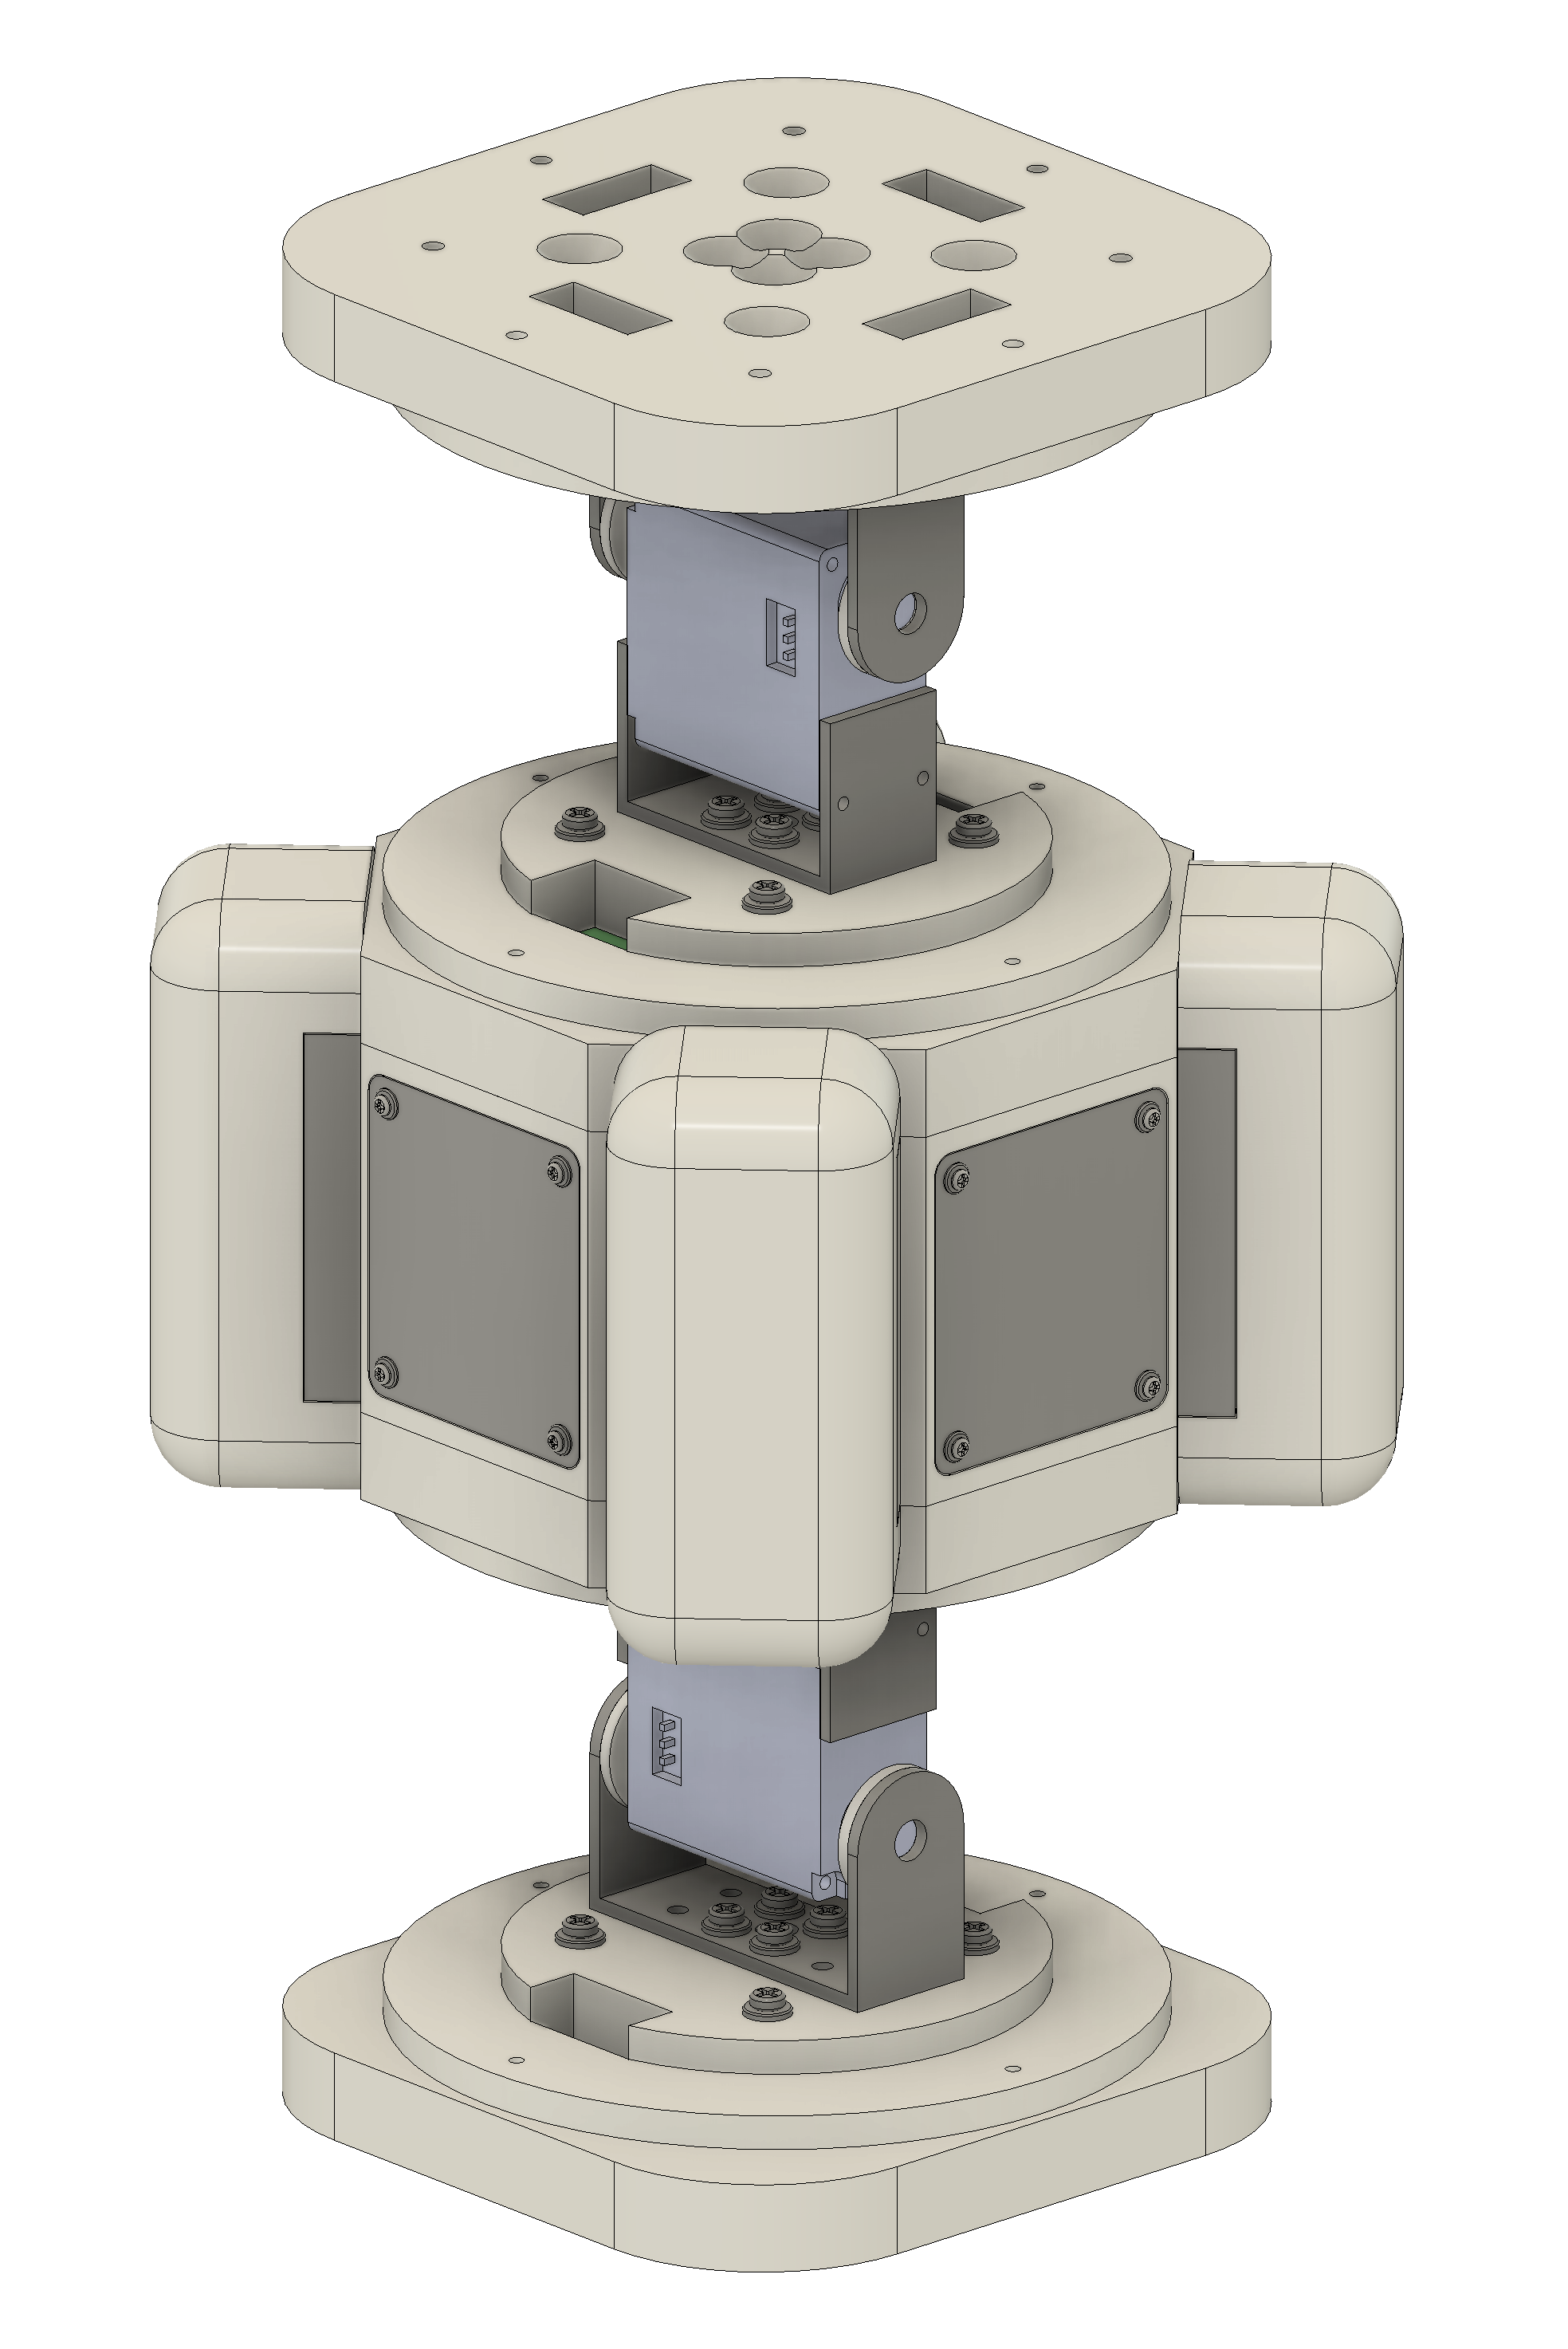
\includegraphics[width=\textwidth]{rysunki/gizmo/module.png}
            \caption{Robot \textit{Gizmo} z założonymi tubami}
            \label{fig: gizmo_module}
        \end{subfigure}
        \hfill
        \begin{subfigure}[b]{0.45\textwidth}
            \centering
            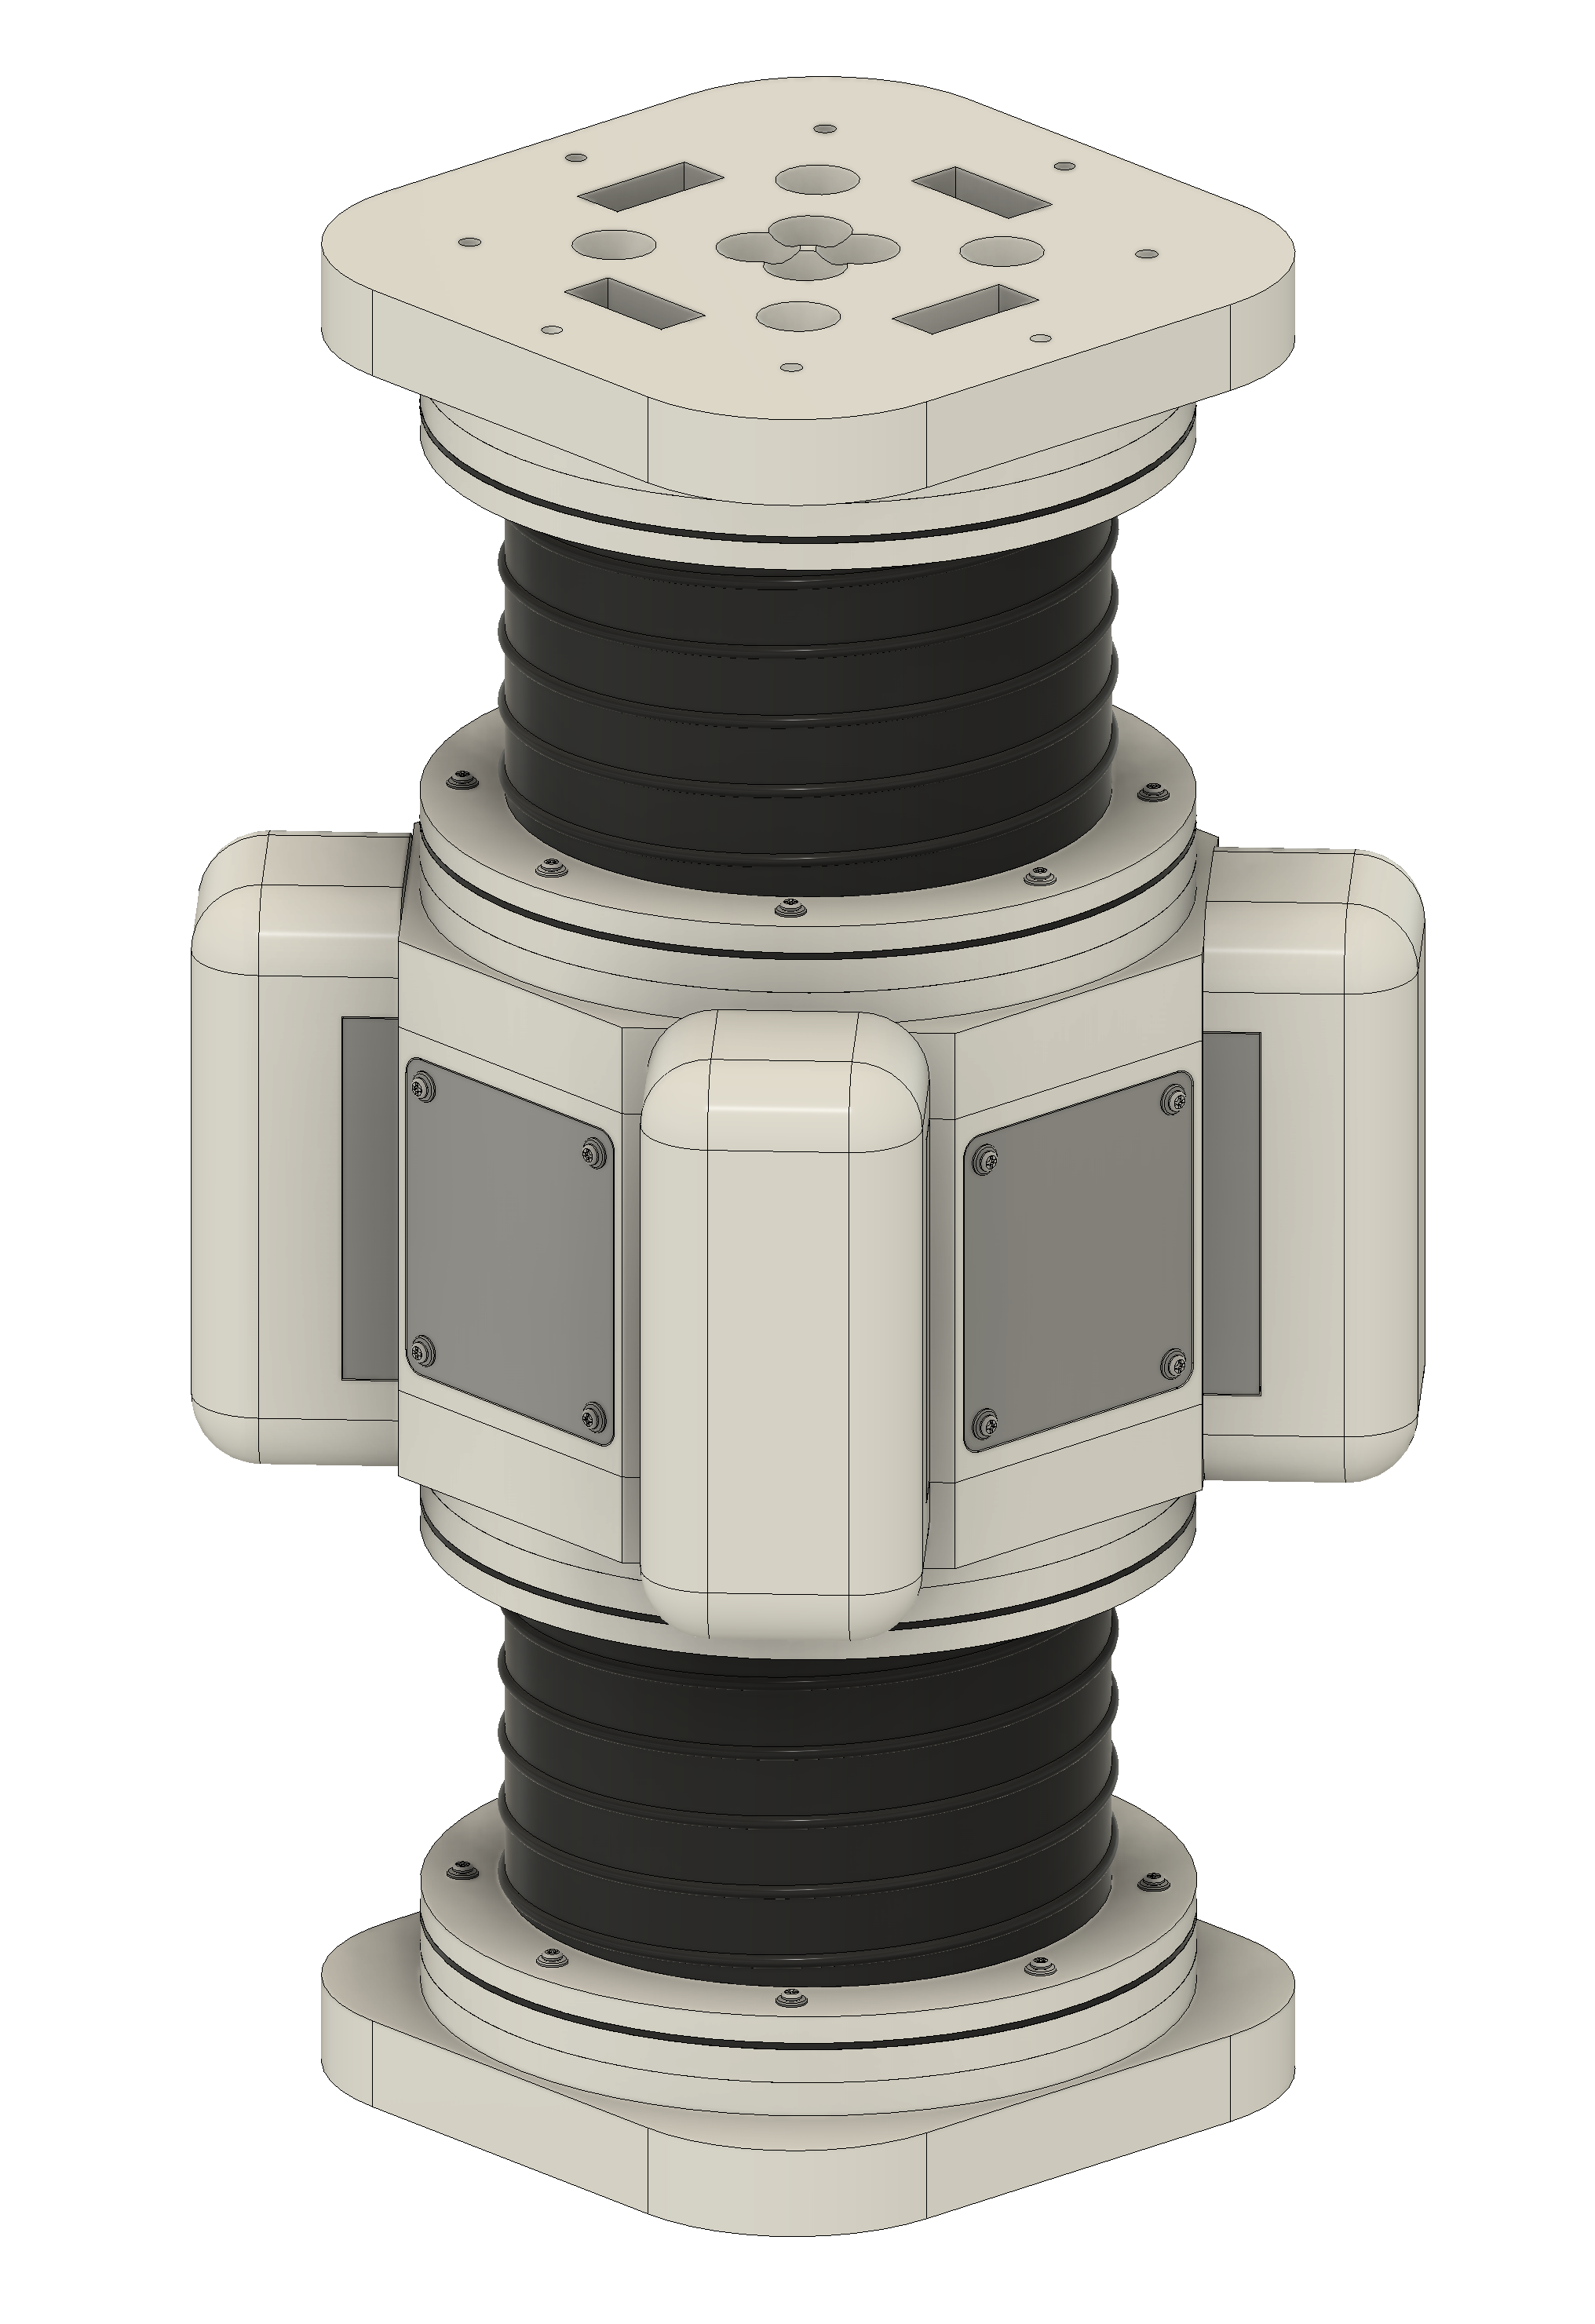
\includegraphics[width=\textwidth]{rysunki/gizmo/module_tube.png}
            \caption{Robot \textit{Gizmo} bez tub}
            \label{fig: gizmo_module_notube}
        \end{subfigure}
    \end{figure} 

Człon sterowania, będący centralnym elementem struktury, jest pusty w środku. Dzięki temu można umieścić w jego wnętrzu płytki PCB oraz oczujnikowanie. Ograniczenia przestrzenne w~kontekście projektu obwodu drukowanego są dość niewielkie -- konstrukcja pozwala na montaż płytki o wymiarach maksymalnych 7x7cm. Jeśli taka powierzchnia nie byłaby wystarczająca, możliwe jest równoległe połączenie kilku takich płytek nakładając je jedna na drugą. Dodatkową przestrzenią użytkową robota stanowią wymienialne panele (szare prostokąty), na których można umieścić np.:~wyświetlacz czy wiatraczek chłodzący wnętrze urządzenia.

Człony ruchowe mają trzy główne funkcje: umożliwienie ruchu, zapewnienie połączenia elektrycznego oraz mechanicznego. Rolę aktuatorów pełnią serwomechanizmy, które jednocześnie są~fizycznym łącznikiem między podstawami robota (konektorami) a członem sterującym. Konektory, widoczne na~końcach urządzenia, posiadają złącza typu gold pin, dając łącznie osiem połączeń elektrycznych. Ich wyprowadzenia służą do uwspólnienia zasilania oraz magistrali komunikacyjnej robota. Ostatnim elementem konstrukcyjnym jest materiałowa tuba, w którą wszyte są przewody. Jej zadaniem jest przekazywanie sygnałów między konektorami a członem sterowania oraz ochrona układu przed ewentualnym pyłem.

\section{Magistrala CAN}
Jedną z priorytetowych kwestii było opracowanie metody komunikacji między modułami. Poszukiwany protokół powinien charakteryzować się:
    \begin{itemize}
        \item Brakiem nadrzędnego urządzenia -- zakłada się, że każdy moduł może zażądać informacji od~innych współpracujących segmentów. Zatem nie może zaistnieć sytuacja, w której protokół zezwala na jedynie jednego zarządcę magistrali. 
        \item Małą ilość przewodów -- ze względu na konstrukcję konektorów niemożliwe jest wyprowadzenie większej liczby pinów, sumarycznie protokół może wykorzystywać cztery z nich (wliczając uziemienie).
        \item Dopuszczalną długością magistrali rzędu kilkudziesięciu metrów -- ważne jest by istniała możliwość dołączenia do jednej magistrali wielu modułów, wiąże się to oczywiście ze~stosunkowo dużą długością linii.
        \item Odpornością na zakłócenia elektromagnetyczne.
    \end{itemize}
Do wyżej wspomnianego profilu pasuje CAN (\textit{Controller Area Network}). Protokół zezwala na~nadawanie przez dowolne urządzenie na magistrali, tak długo jak jest ona wolna lub wysyłana wiadomość ma wyższy priorytet. Maksymalna odległość między krańcowymi węzłami jest zależna od~prędkości transmisji. Dla najwyższej z nich wynoszącej 1 Mb/s, długość magistrali może mieć do 40 m, natomiast dla 50 kb/s dopuszczalna jest odległość aż 1 km \cite{ds102}. Interfejs CANa składa się z dwóch przewodów zazwyczaj sygnowanych jako \texttt{CAN\_H} oraz \texttt{CAN\_L}. Ponieważ protokół wykorzystuje sygnały różnicowe, jest on bardziej odporny na zakłócenia elektromagnetyczne \cite{sloa101} niż typowe magistrale jednostronne (ang \textit{single-ended}).

\subsection{Zasada działania protokołu}
Tak jak wcześniej wspomniano protokół CAN wykorzystuje sygnały różnicowe. Magistrala może być w dwóch stanach: dominującym ($\Delta V = V_{CAN\_H} - V_{CAN\_L} \simeq 2 V$) lub recesywnym ($\Delta V = 0 V$). Co~jest dość nietypowe, logika CANa jest odwrócona w porównaniu ze standardową interpretacją, gdzie dodatnie napięcie stanowi logiczną jedynkę. Przykładowe stany magistrali CAN oraz ich wartości logiczne widoczne są na rysunku \ref{fig: can_bus}.

\begin{figure}[ht!]
    \centering
    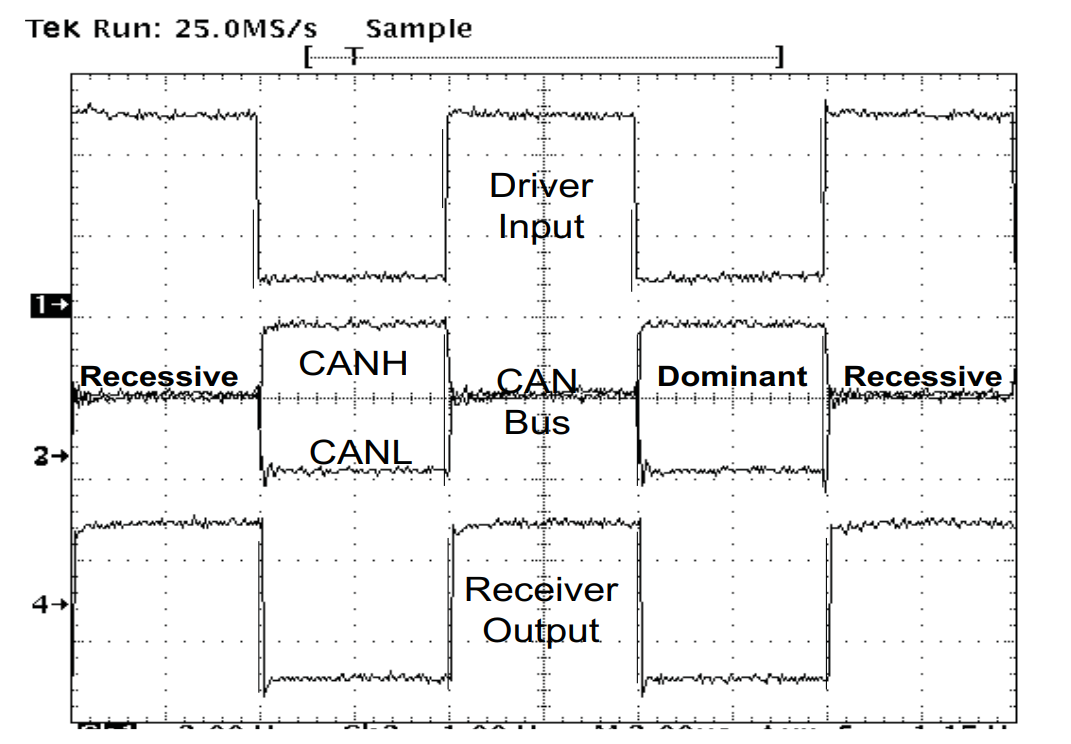
\includegraphics[width=0.7\linewidth]{rysunki/basic_com/can_bus.png}
    \caption{Interpretacja stanów magistrali CAN \cite{sloa101}}
    \label{fig: can_bus}
\end{figure} 

W ramach protokołu możliwe jest wysyłanie 4 rodzajów ramek: danych (ang. \textit{data frame}), błędów (ang. \textit{error frame}), opóźniająca (ang. \textit{overload frame}), żądania (ang. \textit{remote frame}) \cite{can}. Różnice w strukturze wiadomości są dość niewielkie, ale ze względu na użycie w projekcie wyłącznie ramek danych nie zostaną omówione. Poniżej widoczne są pola bitowe ramki danych \ref{frame: can_data_frame}.

\begin{dframe}[!ht]
    \centering
    \begin{bytefield}[endianness=little, bitwidth = 0.0555\linewidth, bitheight = 30pt, boxformatting = {\centering \small}]{5}
        \bitbox{1}{Start} & \bitbox{3}{Pole arbitracji} & \bitbox{1}{RTR} & \bitbox{1}{IDE} & \bitbox{1}{DLC} & \bitbox{4}{Pole danych} & \bitbox{3}{CRC} & \bitbox{1}{ACK} & \bitbox{3}{EOF} \\
    \end{bytefield}
    \caption{\label{frame: can_data_frame} Struktura ramki danych CAN2.0A}
\end{dframe}

\textbf{Bit startu }(logiczne 0), ma za zadanie zasygnalizowanie urządzeniom początku nowej transmisji. Opadające zbocze sygnału pozwala również na synchronizację.

\textbf{Pole arbitracji}, może mieć długość 11 lub 27 bitów zależnie od wybranego formatu (odpowiednio CAN 2.0A oraz CAN 2.0B). Z perspektywy logiki układu stanowi identyfikator wiadomości lub~urządzenia. Jednocześnie w warstwie fizycznej, jego wartość stanowi również o priorytecie wiadomości. 

\textbf{RTR} (ang. \textit{Remote-Transmission-Request}), jednobitowe pole które sygnalizuje czy wysyłana wiadomość zawiera dane (wówczas przyjmuje wartość logicznego 0)

\textbf{IDE} (ang. \textit{Identifier Extenstion Flag}), jednobitowe pole informujące o formacie identyfikatora (logiczne 0 dla CAN 2.0A),

\textbf{DLC} (ang. \textit{Data Length Code}), ma długość 4 bitów a jego wartość wskazuje na ilość wysyłanych bajtów danych. Maksymalna ilość danych, która może zostać przekazana w praktyce wynosi osiem. W przypadku, gdy w polu DLC pojawi się wartość większa, jest ona nadal interpretowana jako osiem \cite{can_spec}.

\textbf{Pole danych} (ang. \textit{data field}), możliwa jest transmisja od zera do ośmiu bajtów danych.

\textbf{Pole sumy kontrolnej CRC} (ang. \textit{CRC -- Cyclic Redundancy Check}), składa się z 15 bitów sumy kontrolnej oraz jednego bitu separującego (logiczna 1)

\textbf{Pole potwierdzenia ACK} (ang. \textit{acknowledge field}), składa się z dwóch bitów. Pierwszy z~nich informuje o poprawności przyjęcia wiadomości przez odbiorniki na magistrali (logiczne 0 przy poprawnej transmisji). Drugi stanowi separację i przyjmuje wartość logicznej jedynki.

\textbf{Pole końcowe EOF} (ang. \textit{end of frame}), składa się z 10 bitów każdy przyjmujący wartość logicznej jedynki.

\subsection{Arbitraż}
W przypadku zaistnienia sytuacji, w której dwa lub więcej urządzeń próbuje nadawać jednocześnie o pierwszeństwie decyduje proces arbitrażu. CAN jako protokół korzysta z mechanizmów zbiorczo nazwanych jako \gls{csma}. Oznacza to, że:
    \begin{itemize}
        \item Magistrala jest dzielona między wieloma równoważnymi węzłami.
        \item Kolizje wykrywane są przez porównywanie stanu magistrali z zawartością, którą chce wysłać dany węzeł -- gdy są one różne oznacza to, że urządzenie przegrało arbitraż.
        \item Wynik arbitrażu dyktowany jest przez priorytet wiadomości -- w przypadku CANa dominującą wartością jest logiczne zero.
    \end{itemize}

Arbitraż występuje na podstawie zawartości pola arbitracji wiadomości.
\begin{dframe}[!ht]
    \begin{tikztimingtable}[%
        timing/dslope=0.05,
        timing/.style={x=4.5ex,y=2ex},
        x=5ex,
        timing/rowdist=6ex,
        timing/name/.style={font=\sffamily\scriptsize}
    ]
        \texttt{Urządzenie 1}   & 1U H 1L 3H 2L 3H 3L 1U \\
        \texttt{Urządzenie 2}   & 1U H 1L 3H 2L 3H 1L {[dotted]1H} 2U \\
        \texttt{Urządzenie 3}   & 1U H 1L 3H 1L {[dotted]1H} 6U \\
        \texttt{Magistrala}     & 1U H 1L 3H 2L 3H 3L 1U\\
        \extracode
        \begin{pgfonlayer}{background}
            \begin{scope}[semitransparent ,semithick]
            \vertlines[darkgray,dotted]{0.5,1.5 ,...,8.0}
            \end{scope}
        \end{pgfonlayer}
    \end{tikztimingtable}
    \caption{\label{fig: arbitraz} Przykładowy przebieg arbitrażu}
\end{dframe}


Powyżej przedstawiono przykładowe rozstrzygniecie arbitrażu \ref{fig: arbitraz} między trzema urządzeniami. Widoczne jest, że w pierwszej kolejności urządzenie 3 przegrywa z 1 oraz 2. Następnie zachodzi podobna sytuacja, gdzie wygrywa urządzenie 1. Stan magistrali jest zawsze zgodny z treścią wiadomości, która wygra arbitraż.

Zrozumienie procesu arbitrażu oraz priorytetyzacji wiadomości jest kluczowe dla komunikacji w sieci wewnętrznej robotów. W przypadku znacznej ilości urządzeń na magistrali istotnie jest, które transmisje będą wysyłane zawsze a które mogą być pominięte. Rozkazy globalne informujące np.: o krytycznych błędach, awaryjnym zatrzymaniu czy prośbie o nadanie identyfikatora, powinny rozpoczynać się od logicznych zer. Należy zwrócić również uwagę, na fakt pewnej nierówności wynikającej z nadawania ''wag'' wiadomościom -- przy zwiększonym ruchu na magistrali może zajść sytuacja, w której wiadomości o niższym priorytecie są zawsze pomijane.

\section{Dobór komponentów elektronicznych}
By zapewnić poprawne funkcjonowanie robota potrzebne jest osiągnięcie symbiozy między projektem bryły i elektroniką. Łatwo wyobrazić sobie sytuację, w której robot ma najwyższej jakości konstrukcję, jednak jego oczujnikowanie nie pozwala na dokładne wysterowanie urządzenia. Analogicznie nawet przy dobrze dobranych elementach elektronicznych, słabe spasowanie komponentów czy ich mała wytrzymałość doprowadzi do niesatysfakcjonującej pracy układu. Zatem wybór elektroniki powinien być warunkowany zarówno budową robota jak i charakterystyką jego pracy.

\subsection{Dobór peryferiów}
Pierwszymi istotnymi peryferiami są serwomechanizmy ST3020 firmy Waveshare \ref{fig: st3020}. Ich dobór warunkowany był wymaganiami mechanicznymi oraz faktem posiadania podzespołów pozwalających na wewnętrzny pomiar kąta obrotu. Wyznaczanie fizycznych parametrów pracy robota takich jak maksymalne momenty siły czy obrotowe nie są elementem tej pracy i zostały przyjęte na~podstawie wniosków wyciągniętych podczas procesu projektowania mechanicznego robota \cite{gizmo}. W przeszłości projektu próbowano opracować metodę wyznaczania kąta obrotu serwomechanizmu w~oparciu o zewnętrzne czujniki. Kwestia ta okazała się nietrywialna w przypadku zrezygnowania ze~stosunkowo drogich enkoderów absolutnych dobrej jakości. Alternatywne podejścia, takie jak użycie czujników Halla w połączeniu z magnesami diametralnie namagnesowanymi czy pomiar w~oparciu o~potencjometr, dawały wyniki obarczone dużym błędem bądź stanowiły metodę pomiaru wymagającą kalibrację każdego z układów. Dlatego zdecydowano się na wybór serwomechanizmu z~wbudowanym układem pomiaru kąta. 

Wybrany serwomechanizm posiada jednak dwie istotne wady: brak dokumentacji technicznej oraz ''głuchą'' komunikację. Pierwsza z nich sprawia, że algorytm pracy serwa jest niejawny oraz nieznane są dokładne parametry podzespołów. Wynikowo należy podejść sceptycznie zarówno do~jakości wysterowania urządzenia jak i pomiaru kąta jego nachylenia. Drugi problem stanowi obsługa serwomechanizmu oparta na komunikacji za pomocą protokołu UART (ang. \textit{universal asynchronous receiver-transmitter}), który nie posiada w swojej formule bitów potwierdzających odbiór wiadomości przez inne urządzenia na magistrali. Jest to słabość, która mogłaby zostać zmitygowana przez odpowiednią strukturę wymiany informacji z urządzeniem, jednak producent nie przewidział takiej możliwości. 

\begin{figure}[ht!]
    \centering
    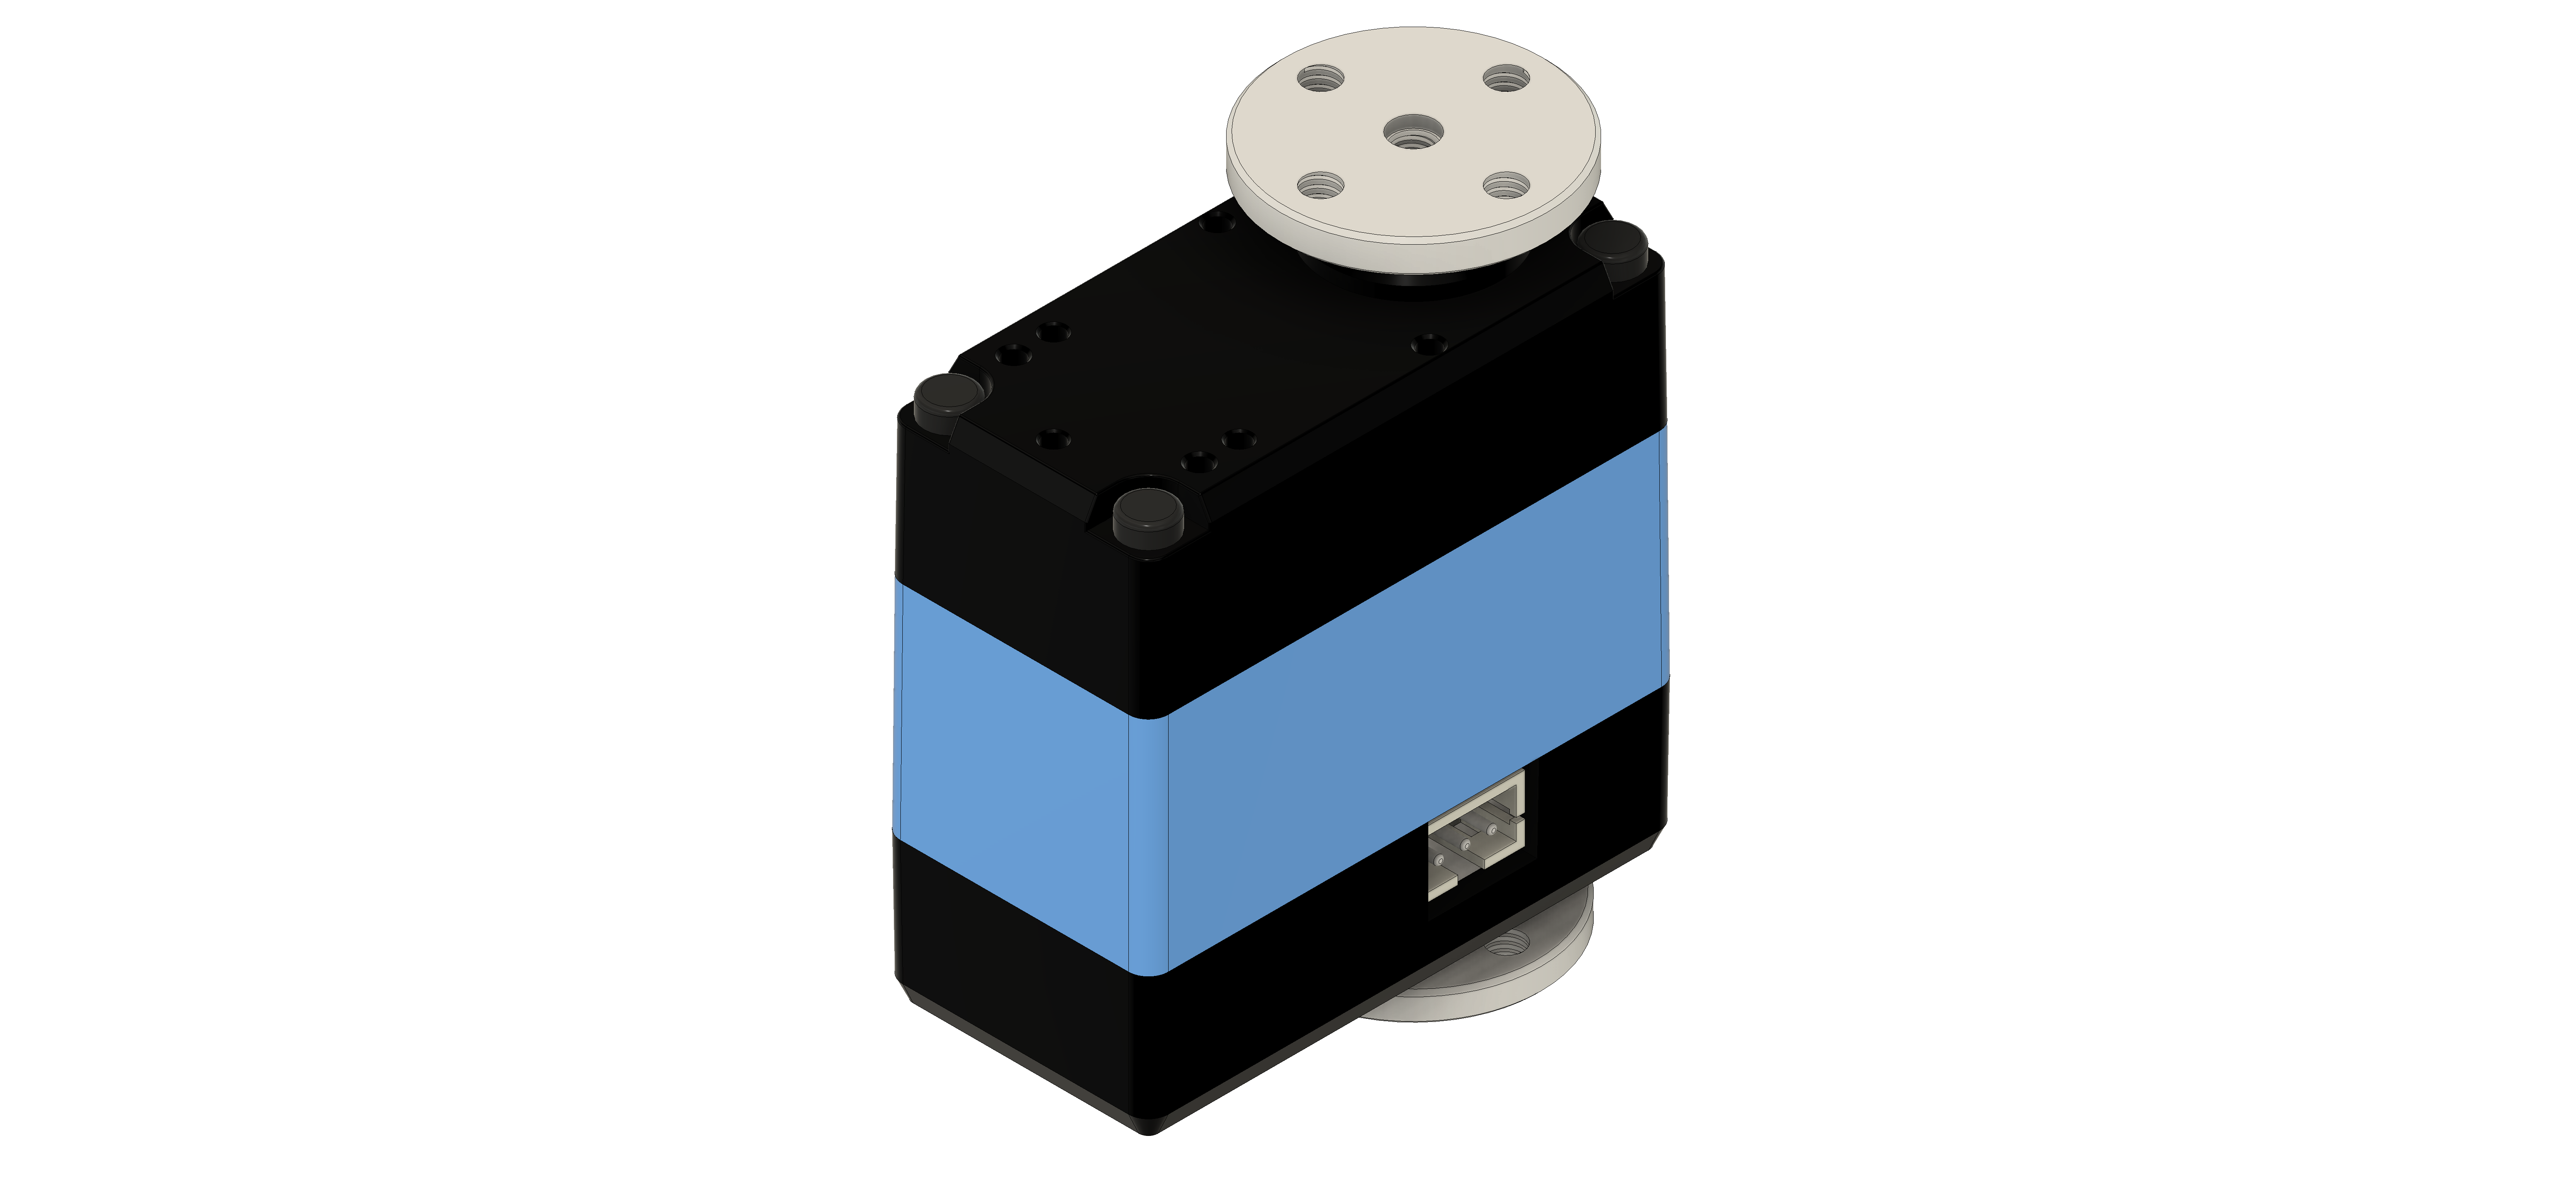
\includegraphics[width=0.7\linewidth]{rysunki/gizmo/ST3020.png}
    \caption{Model serwomechanizmu ST3020 udostępniony przez producenta}
    \label{fig: st3020}
\end{figure} 

Oba te powody złożyły się na decyzję dodania dwóch dodatkowych elementów elektronicznych -- akcelerometrów ADXL345. Dzięki nim możliwe było dokonanie alternatywnego pomiaru kąta obrotu każdego z serwomechanizmów lub pośrednia weryfikacja ich pracy przez pomiar orientacji modułu. Warto dodać, że ze względu na charakter elementu taki pomiar musi być wykonany gdy układ jest statyczny, inaczej wyniki będą zaburzone przez przyśpieszenie samego robota lub drgania mechaniczne związane z jego pracą. W przyszłości akcelerometry mogą zostać również wykorzystane jako sygnalizator kolizji czy jako zabezpieczenie przed zbyt gwałtownym ruchem urządzenia.

Roboty modularne charakteryzują się zdecentralizowaniem informacji, bowiem każdy z modułów jest autonomicznym urządzeniem, a ich stany wewnętrzne choć mogą być przekazywane dalej w~ogólności są niejawne. Oznacza to, że serwisowanie czy diagnostyka problemów w robocie złożonym choćby z kilku modułów może okazać się trudna. Dlatego bardzo istotne jest, by istniała możliwość odtworzenia sekwencji stanów pracy każdego z segmentów. W znacznej mierze jest to problem, który należy rozwiązać oprogramowaniem, jednak nadal wymaga on odpowiedniego wyposażenia robota. Archiwizację umożliwia karta microSD, dzięki której możliwy jest trwały zapis danych. W~założeniu, wszystkie operacje robota powinny być na niej przechowywane. Natomiast obserwację bieżących parametrów pracy robota umożliwia wyświetlacz LCD, który docelowo będzie umieszczony na jednym z wymienialnych paneli członu sterującego. 

\subsection{Dobór mikrokontrolera}
Ostatnim, oraz najważniejszym, elementem wymagającym doboru jest mikroprocesor/mikrokontroler. Wcześniej wspomniane peryferia definiują minimalną ilość oraz rodzaj interfejsów: SDIO (karta microSD), SPI (wyświetlacz), 2x UART (serwomechanizmy), 2x I$^2$C (akcelerometry). Dodatkowo znacznym atutem byłoby posiadanie przez układ wbudowanej obsługi magistrali CAN -- co prawda możliwe jest stosowanie przejściówek, np.: UART-CAN, jednak ułatwiłoby to znacznie proces tworzenia oprogramowania. Biorąc pod uwagę charakter pracy robota, musi mieć on stosunkowo dużą pamięć ROM oraz RAM. Można spodziewać się znacznego obciążenia ze strony głównej magistrali CAN, a także z wykonywania operacji matematycznych opartych o macierze oraz funkcje trygonometryczne -- dotyczących rozwiązywanie zagadnienia kinematyki, kinematyki odwrotnej czy wyliczanie orientacji modułów. Należy również wyjść z założenia, że robot będzie miał dość obszerne oprogramowanie, wynika to z dużej ilości peryferiów do obsłużenia, a także potrzeby implementacji bardziej zaawansowanej logiki systemu.

By przyśpieszyć proces prototypowania modułów zdecydowano się na wykorzystanie gotowej płytki. Analizie poddano trzy rodziny mikrokontrolerów: Arduino, ESP32 oraz STM32. Są to jedne z najpopularniejszych serii płytek na rynku. 

Największą zaletą Arduino jest duże wsparcie ze strony społeczności hobbystów, ale również producentów, którzy zazwyczaj dołączają dedykowane biblioteki obsługujące ich urządzenia. Możliwe jest znalezienie modeli płytek, które spełniałyby oczekiwania związane z pamięciami ROM i RAM a także ilością dostępnych pinów i interfejsów. W porównaniu z innymi produktami w podobnym przedziale cenowym można zauważyć: niższe częstotliwości taktowania zegara (zazwyczaj wynoszące kilkadziesiąt MHz), mniejszą ilość i konfigurowalność przerwań, brak bardziej zaawansowanych funkcji takich jak DMA. Dodatkowym problemem, który ostatecznie zdyskwalifikował użycie Arduino, jest utrudniony proces diagnostyki kodu (ang. \textit{debugging}). Jedynie kilka płytek ma oficjalne wsparcie tej funkcjonalności, w przypadku innych modeli należy użyć zewnętrznych bibliotek.

ESP32 cierpi na podobny problem z debuggingiem, jednak tym razem potrzebny jest zazwyczaj zewnętrzny programator podpinany do pinów JTAG. Powodem odrzucenia tej rodziny mikrokontrolerów jest fakt posiadania zbyt małej ilości pinów.

\begin{figure}[ht!]
    \centering
    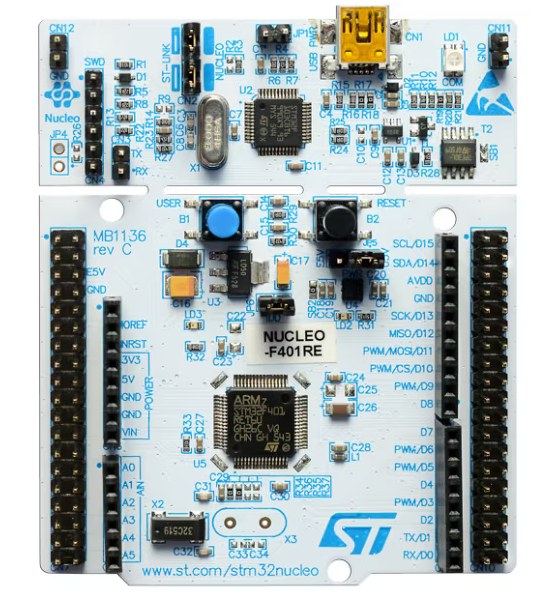
\includegraphics[width=0.4\linewidth]{rysunki/gizmo/nucleo.png}
    \caption{Płytka STM32 Nulceo-F446RE, zdjęcie ze strony producenta}
    \label{fig: stm32}
\end{figure} 

W ofercie STMicroelectronics znajduje się mnogość modeli płytek zróżnicowanych zarówno pod~względem interfejsów jak i ilości dostępnych pinów. Zdecydowano się na rozwiązanie z serii Nucleo, dokładniej Nucleo-F446RE \ref{fig: stm32}. Urządzenie spełnia wymagania wynikające z doboru elementów oraz posiada stosunkowo dużą pamięć RAM (128 kB SRAM) oraz ROM (512 kB flash) \cite{ds1093}. Mikrokontroler ma wbudowane dwa interfejsy magistrali CAN, co stanowi dodatkowy atut. Korzystny jest fakt zapewnienia przez producenta dedykowanego środowiska programistycznego \textit{STM32CubeIDE}, które współpracujące ze wszystkimi produktami tej firmy. Oprogramowanie zaspokaja podstawowe potrzeby związane z pisaniem kodu przeznaczonego dla systemów wbudowanych, zawiera opcje: przechodzenia programu 'krok po kroku', stawiania punktów przerwania czy podglądania zawartości pamięci. Oprócz tego umożliwia prostą konfigurację pinów oraz zegarów urządzenia. Tak jak w~większości układów STM32, możliwy jest debugging wykorzystując wyłącznie połączenie USB z~komputerem hostem. Zasadniczą wadą wyboru rodziny STM32 jest istnienie ograniczonej ilości przykładowych kodów czy gotowych rozwiązań -- wynika to z wyższego progu wejścia w stosunku do platform takich jak Arduino. Dodatkowym kryterium doboru było posiadanie przez mikroprocesor jednostki zmiennoprzecinkowej (ang. \textit{FPU, floating point unit}). Jest to cecha charakterystyczna architektur ARM-Cortex M4 oraz ARM-Cortex M7 \cite{cortexm4}. Jej obecność na pokładzie mikrokontrolera przyśpieszy obliczenia związane z~funkcjami trygonometrycznymi czy macierzami. 